\section{Results}

\begin{frame}{Construction of HD LiDAR Map}
    \begin{figure}
        \centering
        \begin{subfigure}[t]{0.49\textwidth}
            \centering
            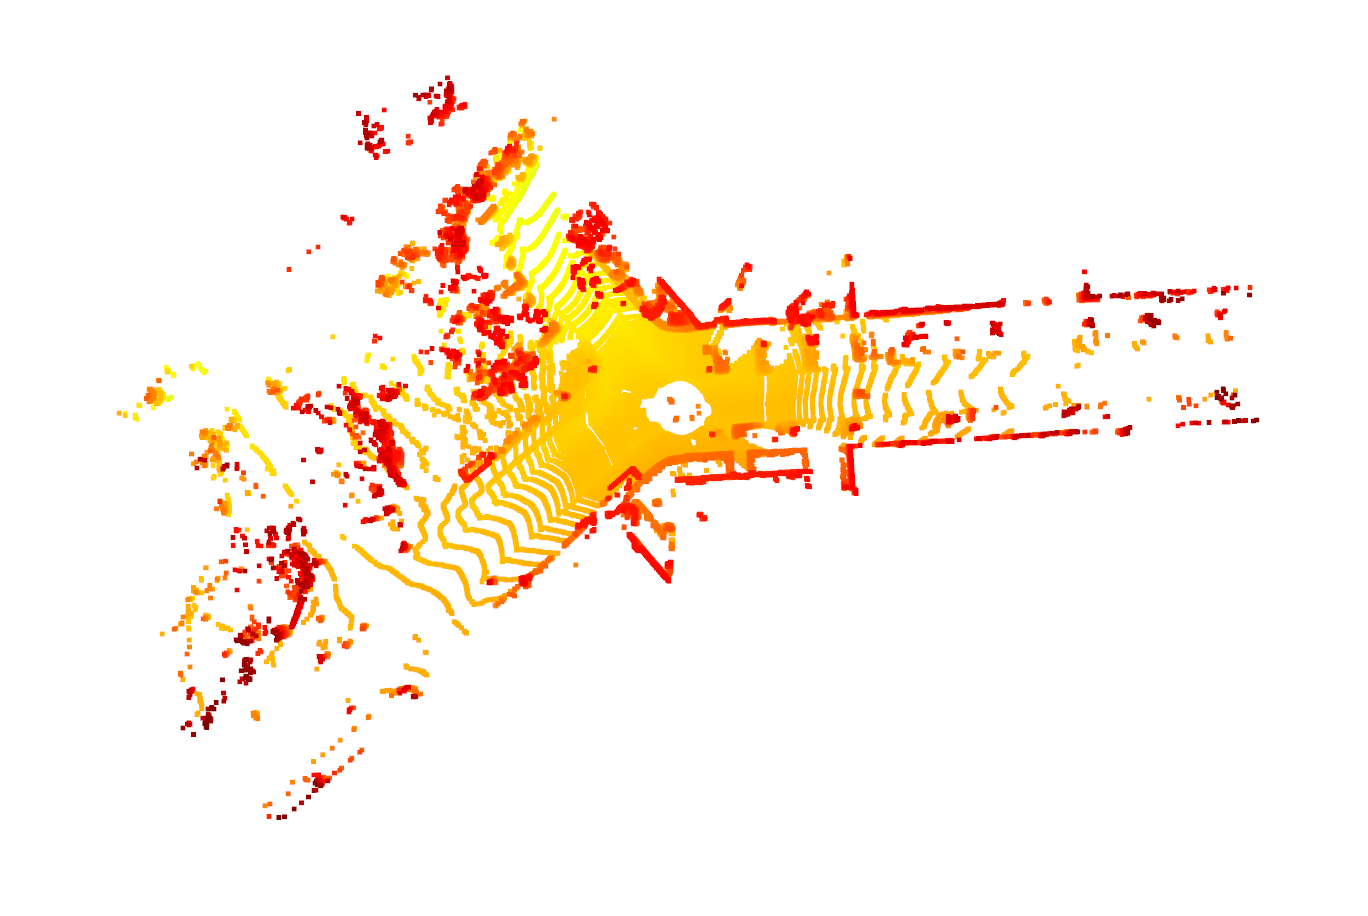
\includegraphics[width=\textwidth]{figures/lidar_frame.png}
            \caption{Sample LiDAR Scan}
        \end{subfigure}
        \hfill
        \begin{subfigure}[t]{0.49\textwidth}
            \centering
            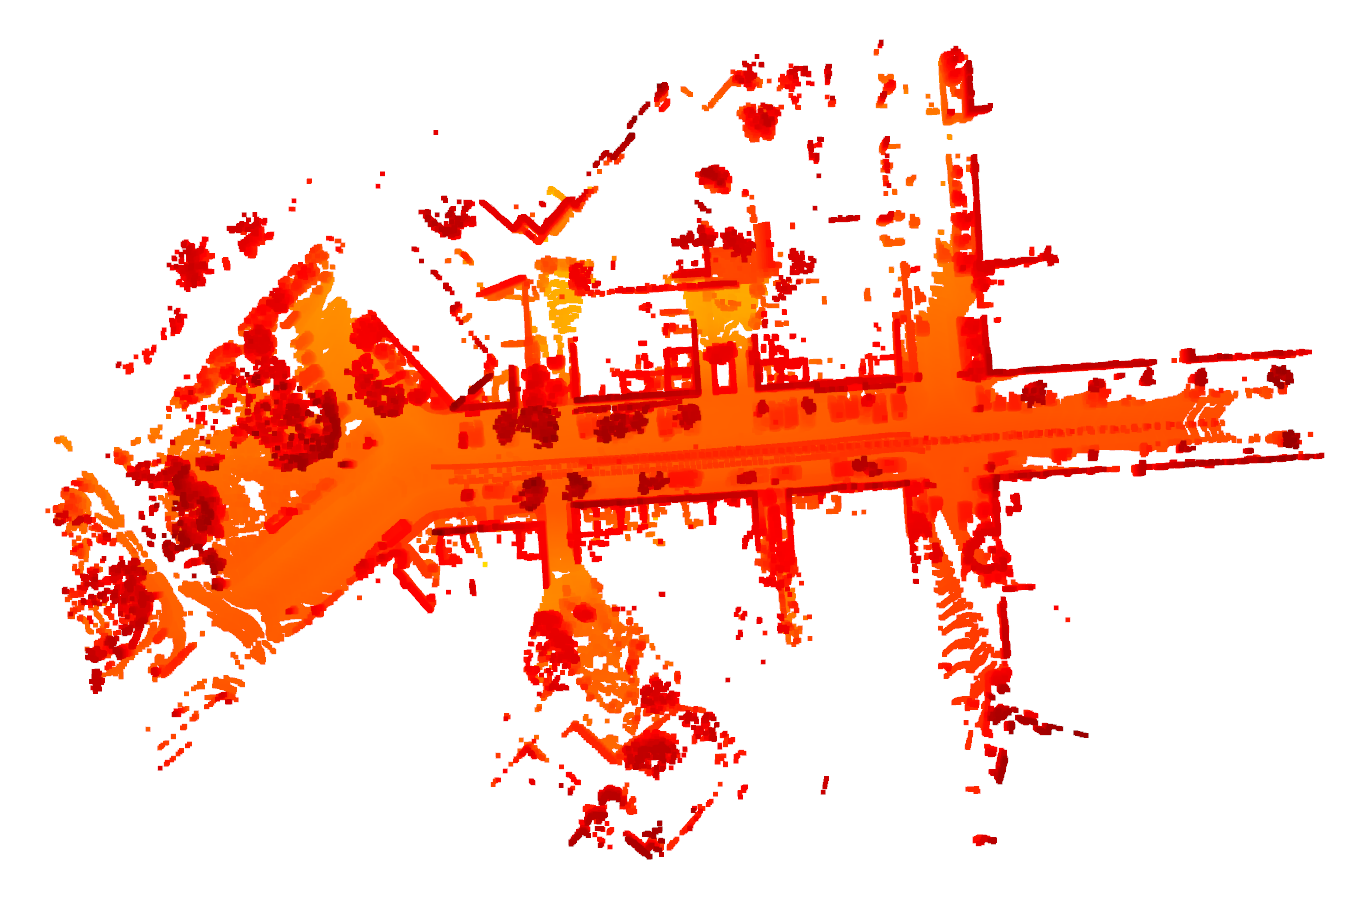
\includegraphics[width=\textwidth]{figures/lidar_map.png}
            \caption{LiDAR Map constructed using ICP}
        \end{subfigure}
    \caption{Sample LiDAR scan and the corresponding LiDAR map constructed using ICP.}
    \end{figure}
\end{frame}

\begin{frame}{Ablation Study for Localization}
\begin{figure}
    \centering
    \begin{subfigure}[t]{0.32\textwidth}
        \centering
        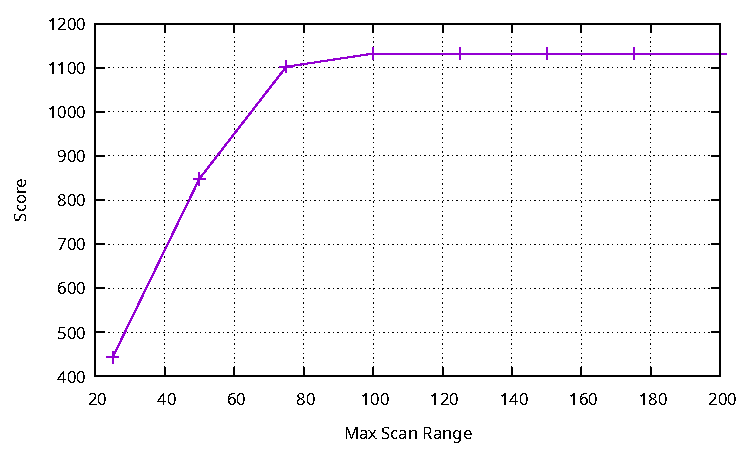
\includegraphics[width=\textwidth]{../02-global-localization/plots/max_scan_range.pdf}
        \caption{Max Scan Range}
    \end{subfigure}
    \begin{subfigure}[t]{0.32\textwidth}
        \centering
        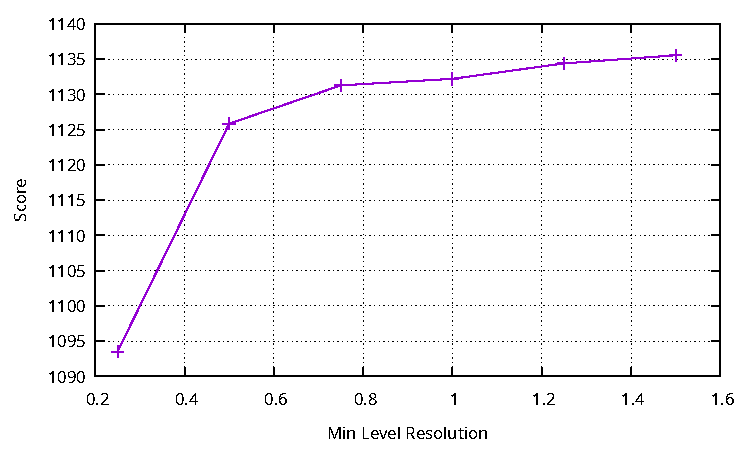
\includegraphics[width=\textwidth]{../02-global-localization/plots/min_level_res.pdf}
        \caption{Min Level Resolution}
    \end{subfigure}
    \begin{subfigure}[t]{0.32\textwidth}
        \centering
        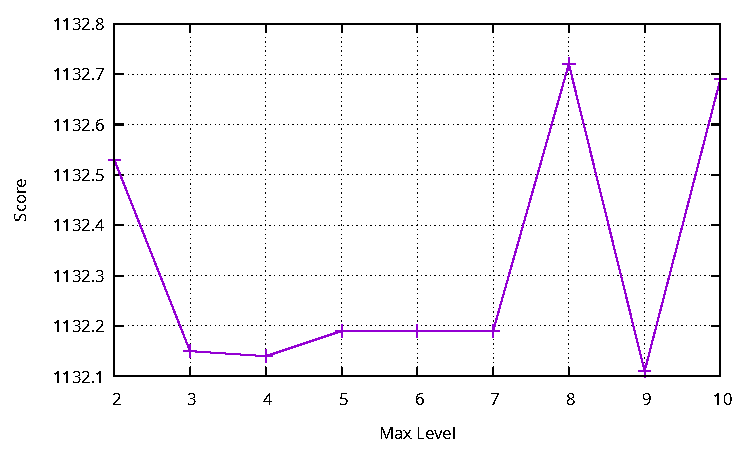
\includegraphics[width=\textwidth]{../02-global-localization/plots/max_level.pdf}
        \caption{Max Level}
    \end{subfigure}
    \begin{subfigure}[t]{0.32\textwidth}
        \centering
        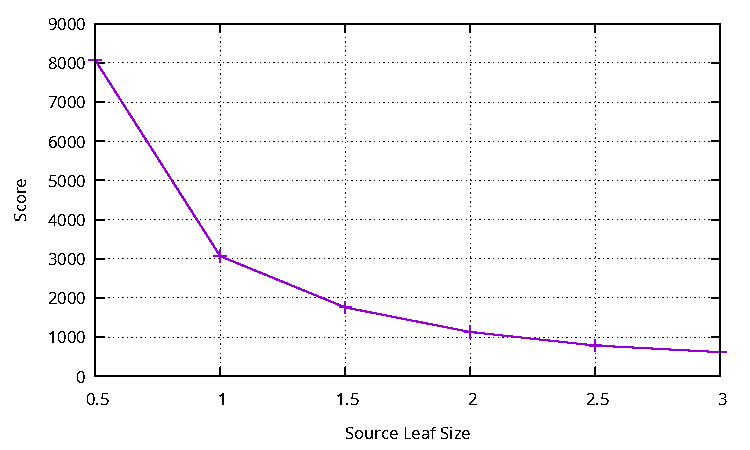
\includegraphics[width=\textwidth]{../02-global-localization/plots/src_leaf_size.pdf}
        \caption{Source Leaf Size}
    \end{subfigure}
    \begin{subfigure}[t]{0.32\textwidth}
        \centering
        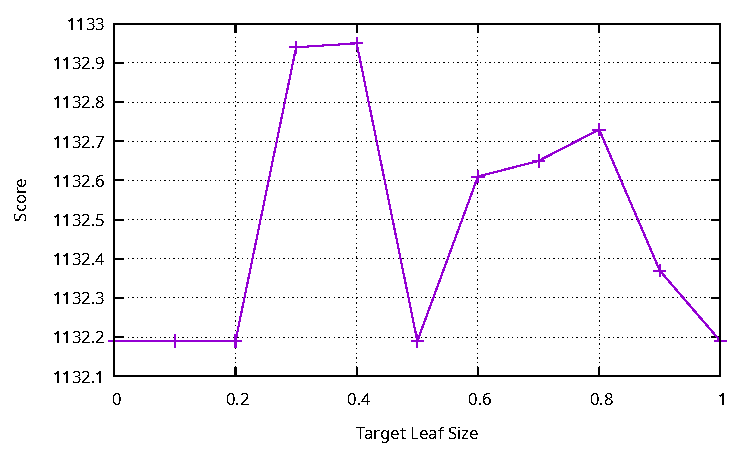
\includegraphics[width=\textwidth]{../02-global-localization/plots/tar_leaf_size.pdf}
        \caption{Target Leaf Size}
    \end{subfigure}
    \caption{Change in localization score with variation of parameters in 3D-BBS.}
\end{figure}
\end{frame}

\begin{frame}{Image to 3D Projection}
\begin{figure}
    \centering
    \begin{subfigure}[t]{0.49\textwidth}
        \centering
        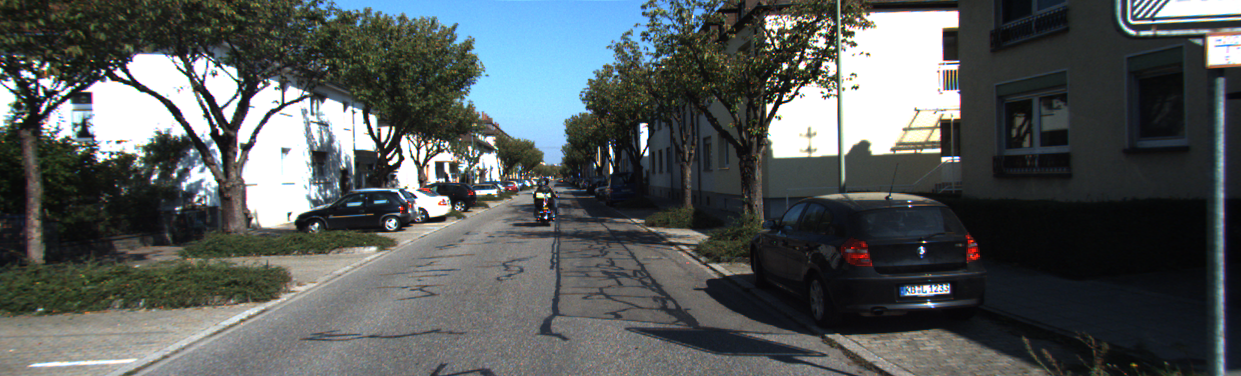
\includegraphics[width=\textwidth]{figures/rgb_image.png}
        \caption{Sample RGB Image}
    \end{subfigure}
    \begin{subfigure}[t]{0.49\textwidth}
        \centering
        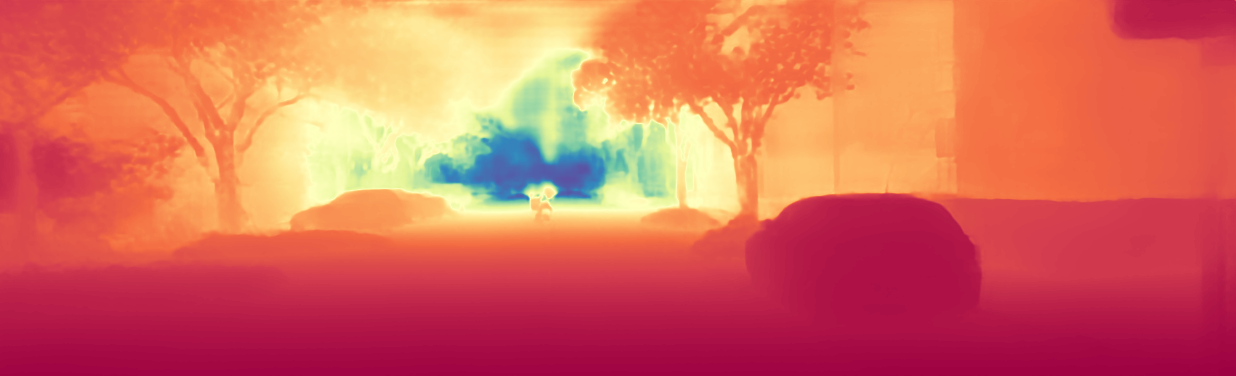
\includegraphics[width=\textwidth]{figures/depth_estimate.png}
        \caption{Metric Depth Estimate}
    \end{subfigure}
    \begin{subfigure}[t]{0.49\textwidth}
        \centering
        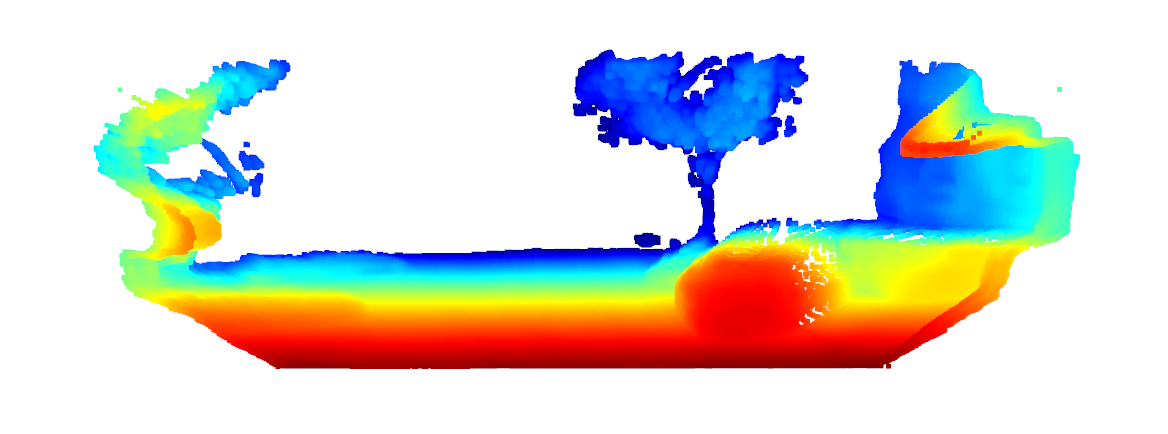
\includegraphics[width=\textwidth]{figures/projected_point_cloud.png}
        \caption{Projected Point Cloud}
    \end{subfigure}
    \begin{subfigure}[t]{0.49\textwidth}
        \centering
        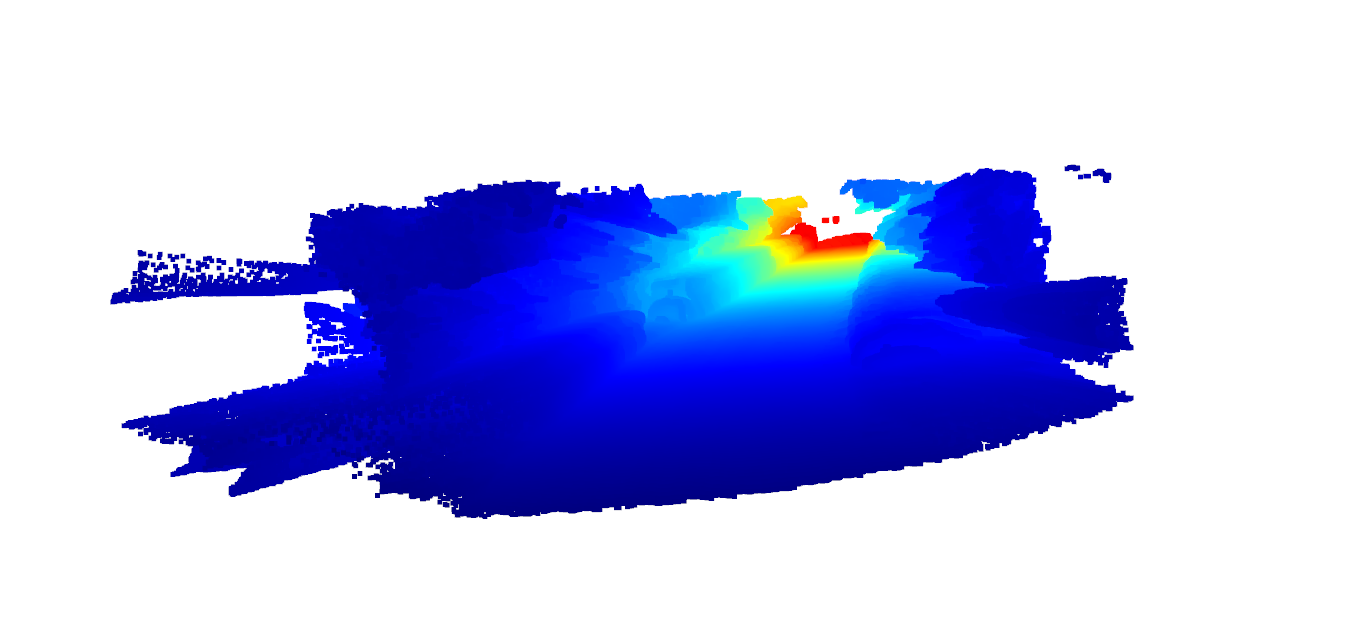
\includegraphics[width=\textwidth]{figures/concatenated_point_cloud.png}
        \caption{Concatenated Point Cloud}
    \end{subfigure}
    \caption{Reprojection from the image to 3D space, using depth estimatation.}
\end{figure}
\end{frame}
